\documentclass[a4paper,4pt]{book}
\usepackage{ctex}
\usepackage{fontenc}
\usepackage{changepage}
\usepackage{amsmath,amsthm}
\usepackage{amssymb}
\usepackage[utf8]{inputenc}
\usepackage{lmodern}
\usepackage{hyperref}
\usepackage{graphicx}
\usepackage{enumerate}
\usepackage[english]{babel}
\usepackage{amsmath}
\usepackage{amssymb}
\usepackage{latexsym}
\usepackage{multirow}
\usepackage{bigdelim}
\usepackage{color}
\usepackage{graphicx}
\usepackage{wrapfig}
\usepackage{picinpar}
\usepackage{picins}
\usepackage{float}
\usepackage{clrscode}
\usepackage{algorithm} %format of the algorithm
\usepackage{algorithmic} %format of the algorithm
\usepackage{subfigure}
\usepackage{xeCJK}
\usepackage{varwidth}
\usepackage{caption}
\setCJKmainfont{宋体}
\setmainfont{宋体}
\setmonofont{Courier New} % 等寬字型
\XeTeXlinebreakskip = 0pt plus 1pt minus 0.1pt
\newfontfamily{\H}{黑体}
\newfontfamily{\K}{楷体}
\newfontfamily{\S}{黑体}
\captionsetup[figure]{name=图}
%%%%%%%%%%%%%%%%%%%%%%%%%%%%%%%%%%%%%%%%%%%%%%%%%%%%%%%%%%%%%%%%%%%%%%%%%%%%%%%%
% 'dedication' environment: To add a dedication paragraph at the start of book %
% Source: http://www.tug.org/pipermail/texhax/2010-June/015184.html            %
%%%%%%%%%%%%%%%%%%%%%%%%%%%%%%%%%%%%%%%%%%%%%%%%%%%%%%%%%%%%%%%%%%%%%%%%%%%%%%%%
\newenvironment{dedication}
{
   \cleardoublepage
   \thispagestyle{empty}
   \vspace*{\stretch{1}}
   \hfill\begin{minipage}[t]{0.66\textwidth}
   \raggedright
}
{
   \end{minipage}
   \vspace*{\stretch{3}}
   \clearpage
}

%%%%%%%%%%%%%%%%%%%%%%%%%%%%%%%%%%%%%%%%%%%%%%%%
% Chapter quote at the start of chapter        %
% Source: http://tex.stackexchange.com/a/53380 %
%%%%%%%%%%%%%%%%%%%%%%%%%%%%%%%%%%%%%%%%%%%%%%%%
\makeatletter
\renewcommand{\@chapapp}{}% Not necessary...
\newenvironment{chapquote}[2][2em]
  {\setlength{\@tempdima}{#1}%
   \def\chapquote@author{#2}%
   \parshape 1 \@tempdima \dimexpr\textwidth-2\@tempdima\relax%
   \itshape}
  {\par\normalfont\hfill--\ \chapquote@author\hspace*{\@tempdima}\par\bigskip}
\makeatother
\newtheorem{theorem}{\textbf{定理}}[section]
\newtheorem{defination}{\textbf{定义}}[section]
\newtheorem{coro}{\textbf{推论}}[section]
\newtheorem{sample}{\textbf{例}}[section]
\newtheorem{guess}{\textbf{猜想}}[section]
\renewcommand{\figurename}{图}
\floatname{algorithm}{算法}
\renewcommand{\algorithmicrequire}{\textbf{输入:}}
\renewcommand{\algorithmicensure}{\textbf{输出:}}
\begin{document}
\pagestyle{plain}  %取消页码
\chapter{基本概念}
%%第一章的内容
\chapter{道路与回路}
\section{道路与回路}
\begin{defination}\K 有向图G=(V,E)中,若边序列P=($e_{i1},e_{i2},\dots,e_{iq}$ ),其中$e_{ik}=(v_l,v_j )$ 满足$v_l$ 是$e_{ik-1}$的终点,$v_j$是$e_{ik+1}$的始点,就称P 是G 的一条\textbf{有向道路}。如果$e_{iq}$的终点也是$e_{i1}$的始点,则称P 是G的一条\textbf{有向回路}。
\end{defination}
\begin{figure}[H]
  \centering
  % Requires \usepackage{graphicx}
  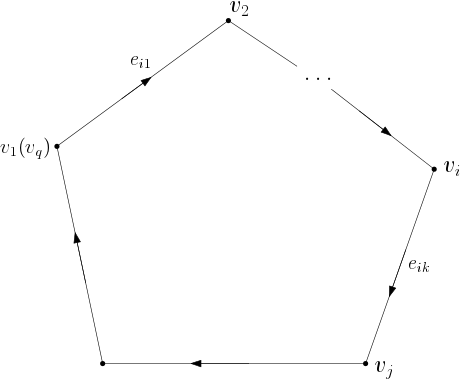
\includegraphics[width=0.5\textwidth]{2.1.1.png}\\
  \caption*{一条有向的回路}
\end{figure}

\begin{sample}\H 下图中,边序列($e_5,e_4,e_5,e_7$ )是有向道路,($e_5,e_4,e_5,e_7,e_3$ )是有向回路。($e_5,e_4,e_1,e_2$ ) 是简单有向道路,($e_5,e_4,e_1,e_2,e_3$ ) 是简单有向回路。($e_1,e_2$ )是初级有向道路,($e_1,e_2,e_3$ )是初级有向回路。
\begin{figure}[H]
  \centering
  % Requires \usepackage{graphicx}
  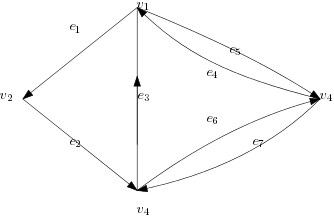
\includegraphics[width=0.5\textwidth]{2.1.png}\\
\caption{}\label{fig:2.1}
\end{figure}
\end{sample}
\begin{defination}\K
无向图G=(V,E)中,若点边交替序列P=$(v_{i1},e_{i1},v_{i2},e_{i2},\dots,e_{iq-1},v_{iq} )$满足$v_{ik}$,$v_{ik+1}$是$e_{ik}$ 的两个端点,则称P是G中的一条链,或道路。如果$v_{iq}=v_{i1}$,则称P 是G 中的一个圈,或\textbf{回路}。\\
如果P中没有重复出现的边,称之为\textbf{简单道路}或\textbf{简单回路},若其中结点也不重复,又称之为\textbf{初级道路}或\textbf{初级回路}。
\end{defination}
\textbf{思考}非初级有向道路的简单有向道路有什么特征?
\begin{sample}\H
下图中边序列($e_4,e_5,e_4,e_6$ )是道路,($e_4,e_5,e_4,e_6,e_3$ )是回路;($e_4,e_5,e_1,e_2$ )是简单道路,($e_4,e_5,e_1,e_2,e_3$ )是简单回路;($e_1,e_2$ )是初级道路,($e_1,e_2,e_3$ ) 是初级回路。
\begin{figure}[H]
  \centering
  % Requires \usepackage{graphicx}
  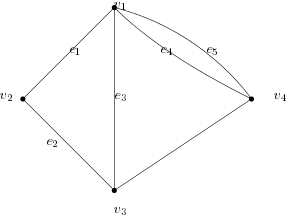
\includegraphics[width=0.5\textwidth]{2.2.png}\\
\caption{}\label{fig:2.2}
\end{figure}
\end{sample}
\begin{sample}
\H 设C是简单图G中含结点数大于3的一个初级回路,如果结点$v_i$和$v_j$在C中不相邻,而边($v_i,v_j$ )∈E(G),则称($v_i,v_j $) 是C的一条弦。若对每一个$v_k∈V(G)$,都有d($v_k$ )≥3,则G中必含带弦的回路。
\begin{adjustwidth}{0.62cm}{0.62cm}
\textbf{证明:}\S {在G中构造一条极长的初级道路$P=(e_{i1},e_{i2},\dots,e_{iq} )$,不妨设$e_{i1}=(v_0,v_1 )$,$e_{il}=(v_{l-1},v_l )$。由于P是极长的初级道路,所以$v_0$ 和$v_1$ 的邻接点都在该道路P上。由已知条件,d($v_0$ )≥3,不妨设Γ($v_0$ )={$v_1,v_{ij},v_{ik},\dots$}。其中1<j<k,这时($v_0,v_1,\dots,v_{i},v_0$ )是一条初级回路,而($v_0,v_{ij}$ ) 就是该回路中的一条弦。}
 \end{adjustwidth}
\end{sample}
% 改编到教材11页
\begin{sample}
设C是简单图G中含结点数大于3的一个初级回路,如果结点$v_i$和$v_j$在C中不相邻,而边($v_i,v_j$ )∈E(G),则称($v_i,v_j$ ) 是C 的一条弦。若对每一个$v_k$∈V(G),都有d($v_k$)≥3,则G 中必含带弦的回路。
\begin{adjustwidth}{0.62cm}{0.62cm}
\textbf{证明 :}在G中构造一条极长的初级道路P=($e_{i1},e_{i2},\dots,e_{iq}$ ),不妨设$e_{i1}$=($v_0,v_1$ ),$e_{il}=(v_{l-1},v_l $)。由于P是极长的初级道路,所以$v_0$ 和$v_1$ 的邻接点都在该道路P上。由已知条件,d($v_0$)≥3,不妨设Γ($v_0$)={$v_1,v_{ij},v_{ik},\dots$}。其中1<j<k,这时($v_0,v_1,\dots,v_{ik},v_0$ )是一条初级回路,而($v_0,v_{ij}$ ) 就是该回路中的一条弦。
\end{adjustwidth}
\end{sample}
\begin{sample}
设G=(V,E)是无向图,如果V(G)可以划分为子集X和Y,使得对所有的e=(u,v)∈E(G),u和v都分属于X和Y,则称G是二分图。证明:如果二分图G中存在回路,则它们都是由偶数条边组成的。
\begin{adjustwidth}{0.62cm}{0.62cm}
\textbf{证明:}设C是二分图G的任一回路,不妨设$v_0$∈X是C的始点,由于G是二分图, 所以沿回路C 必须经过偶数条边才能达到某结点$v_i$∈X,因而只有经过偶数边才能回到$v_0$
\end{adjustwidth}
\end{sample}
\begin{defination}\K
 设G是无向图,若G的任意两结点之间都存在道路,就称G是\textbf{连通图},否则称为\textbf{非连通图}。\\
 如果G是有向图,不考虑其边的方向,即视之为\textbf{无向图},若它是连通的,则称G是连通图。\\
若连通子图H不是G的任何连通子图的真子图,则称H是G的\textbf{极大连通子图},或称\textbf{连通支}。显然G的每个连通支都是它的\textbf{导出子图}。
\end{defination}
\begin{sample}
图2.1和图2.2都是连通图,图2.3是非连通图。其中(a)有两个连通支, 它们的结点集分别是{$v_1,v_2,v_3$ }和{$v_4,v_5$ },(b)有三个连通支,其结点集是{$v_1,v_2,v_3$ },{$v_4,v_5$ } 和{$v_6$ }。
\end{sample}
\begin{figure}
  \centering
  \begin{minipage}[!ht]{.5\linewidth}
  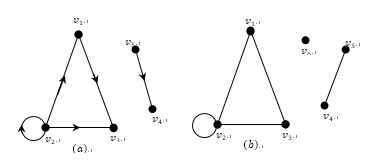
\includegraphics[width=1.0\linewidth]{2.3.png}
  \caption{}
  \end{minipage}
  \begin{minipage}[!ht]{.35\linewidth}
   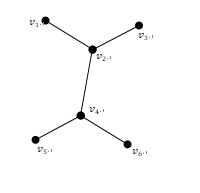
\includegraphics[width=1.0\linewidth]{2.4.png}
  \caption{}
  \end{minipage}
\end{figure}
\begin{sample}
图2.4是连通图,它不含回路,而且在任意两结点之间都只有唯一的一条初级道路。这种图称为树,它是含边数最少的连通图。
\end{sample}
\begin{sample}
设G是简单图,证明当m=1/2 (n-1)(n-2)时,G是连通图。
\begin{adjustwidth}{0.62cm}{0.62cm}
\textbf{证明:}假定G是非连通图,则至少含有2个连通支。设分别为$G_1=(V_1,E_1)$,$G_2=(V_2,E_2)$。其中$|V_1 (G_1 )|=n_1$,$|V_2 (G_2 )|=n_2$。$n_1+n_2=n$。由于G是简单图,因此$$|E_1 (G_1 )|\leq1/2 n_1(n_1-1)$$$$|E_2 (G_2 )|\leq1/2 n_2 (n_2-1)$$$$m\leq1/2 n_1(n_1-1)+1/2 n_2(n_2-1)$$\\
由于$n_1$≤n-1,$n_2$≤n-1,\\
所以$$m\leq1/2 (n-1)(n_1-1+n_2-1)$$$$=1/2 (n-1)(n-2)$$\\
与已知条件矛盾,故G是连通图。
%
\end{adjustwidth}
\end{sample}

\section{道路与回路的判定}
\paragraph{}通常可以利用邻接矩阵或搜索法判定某个图G的两结点间是否存在道路,或者判定它是否连通。首先介绍\textbf{ 邻接矩阵}的判定方法。
\paragraph{}设$A=(a_{ij})_{n\times n}$是G的邻接矩阵。由A的定义,$a_{ij}=1$表示$(v_i,v_j )\in E(G)$,即$v_i$可以通过某条边e到达$v_j$,者说G中有道路从$v_i$到$v_j$。根据矩阵乘法,设$A^2=(a_{ij}^{(2)})$,有
\begin{displaymath}
a_{ij}^{(2)}=\sum_{k=1}^{n}a_{ik}.a_{kj}
\end{displaymath}
$a_{ij}^{(2)}\neq 0$当且仅当存在k,使$a_{ik}=a_{kj}=1$。也就是说,如果G中存在结点$v_k$,满足$(v_i,v_k )$,$(v_i,v_k )\in E(G)$,即经过2条边$(v_i,v_k)$,$(v_k,v_j)$,$v_i$可以到达$v_j$时,$a_{ij}^{(2)}\neq 0$。同理,$A^l(l≤n)$中的元素$a_{ij}^{(l)}\neq0$表示了$v_i$可以经过l条边到达$v_j$。因此令$$P=A+A_2+\cdots+A_n,$$如果$p_{ij}=t$,说明$v_i$有t条道路可以到达$v_j$。若$p_{ij}=0$,即n步之内$v_i$不能到达$v_j$,则在G中不存在$v_i$到$v_j$ 的路。否则,若$v_i$ 经过l(l≤n) 步可达$v_j$,由\textbf{抽屉原理},该道路上一定存在重复出现的结点$v_k$,而$v_k$之间的这段路C 是一个回路。删去这段回路$v_i$ 仍然可达$v_j$。由于G中只存在n个不同的结点,所以只要$v_i$有道路到$v_j$,一定有$p_{ij}≠0$。
\paragraph{}在许多实际问题中,往往只要求了解$v_i$与$v_j$之间是否存在道路。对此可以采用逻辑运算的方法,即$$a_{ij}^{(l)}=\bigvee_{k=1}^{n}(a_{ik}^{(l-1)}\bigwedge a_{ij}),l=2,3,\cdots,n。$$相应地,$$P=A\bigvee A^2 \bigvee \cdots \bigvee A^n$$就是图G的道路矩阵。
\paragraph{}用上述方法求G的道路矩阵,计算复杂性为Ο($n^4$ )。以下介绍的Warshall算法是一个更好的方法,其计算复杂性是Ο($n^3$)。
\begin{adjustwidth}{0.62cm}{0.62cm}
\textbf{Warshall算法}\\
begin\\
\begin{enumerate}
\item $P\leftarrow A$,
\item for i=1 to n do
\item \quad for j=1 to n do
\item \qquad for k=1 to n do\\ \indent\quad$p_{jk}\leftarrow p_{jk}\bigvee(p_{jk}\bigwedge p_{ik})$。
\end{enumerate}
\end{adjustwidth}
\begin{sample}
采用Warshall算法计算图2.5道路矩阵的过程是:\\
$P\leftarrow
\begin{bmatrix}
0&1&1&0&0\\
0&0&1&1&0\\
0&0&0&0&1\\
0&0&0&0&0\\
1&0&0&1&0\\
\end{bmatrix}
$\\
$P(i=1)=\begin{bmatrix}
0&1&1&0&0\\
0&0&1&1&0\\
0&0&0&0&1\\
0&0&0&0&0\\
1&1&1&1&0\\
\end{bmatrix}\quad P(i=2)= \begin{bmatrix}
0&1&1&1&0\\
0&0&1&1&0\\
0&0&0&0&1\\
0&0&0&0&0\\
1&1&1&1&0\\
\end{bmatrix}
$\\
$P(i=3)=\begin{bmatrix}
0&1&1&1&1\\
0&0&1&1&1\\
0&0&0&0&1\\
0&0&0&0&0\\
1&1&1&1&1\\
\end{bmatrix}\quad P(i=4)=P(i=3),
$\\
\begin{figure}[h]
\vspace{-50pt}
\parbox[t]{0.5\textwidth}{$
P(i=5)=\begin{bmatrix}
1&1&1&1&1\\
1&1&1&1&1\\
1&1&1&1&1\\
0&0&0&0&0\\
1&1&1&1&1\\
\end{bmatrix}$}
\centering
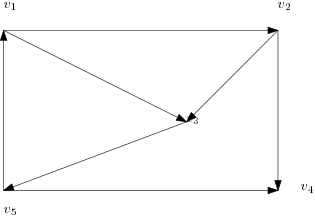
\includegraphics[width=0.4\textwidth]{2.5.png}%
\captionsetup{margin=3em}
\caption{}
\vspace{-30pt}
\end{figure}
\end{sample}
\begin{theorem}\K Warshall算法的结果是图G的道路矩阵。
\end{theorem}
\textbf{证明:}该定理的严格证明需要对三层循环分别使用归纳法。现只证其最外层循环。\\
基始:当i=1时,\\
$p_{jk}^{(l)}=p_{jk}\bigvee (p_{jl}\bigwedge p_{lk}),k=1,2,\cdots,n;j=1,2,\cdots,n$\\
$p_{jk}^{(1)}=1$当且仅当$p_{jk}=1$或$p_{j1}=p_{1k}=1$,其中$p_{jk}=1$表明$v_j$直接可达$v_k$,$p_{j1}=p_{1k}=1$表明$v_j$直接经过$v_1$可达$v_k$。因此$p_{jk}^{(l) }=1$ 当且仅当结点集{$v_j,v_1,v_k$ } 之间有$v_j$到$v_k$的路。\\
 \indent i=2时,$p_{jk}^{(2)}=p_{jk}^{(1)}∨(p_{j2}^{(1)}∧p_{2k}^{(1)})$,$k=1,2,\cdots,n$;$j=1,2,\cdots,n$。$p_{jk}^{(2)}=1$当且仅当$p_{jk}^{(1)}=1$或$ p_{j2}^{(1)}=p_{2k}^{(1)} =1$,其中$p_{jk}^{(1)}=1$表明结点集{$v_j,v_1,v_k$ }之间有$v_j$到$v_k$的道路;$p_{j2}^{(1)} $和$p_{2k}^{(1)}$为1表明{$v_j,v_1,v_2,v_k $} 之间$v_j$有必通过$v_2$到达$v_k$的道路,因此,$p_{jk}^{(2)}=1$当且仅当结点集{$v_j,v_1,v_2,v_k $}中有$v_j$到$v_k$的道路。\\
\indent 设i=n-1时,$p_{jk}^{(n-1)}=1$当且仅当结点集{$v_j,v_1,v_2,\cdots,v_{n-1},v_k$}之中有$v_j$到$v_k$的道路。\\
\indent 则i=n时,$p_{jk}^{(n)}=p_{jk}^{(n-1)}\bigvee(p_{jn}^{(n-1)}\bigwedge p_{nk}^{(n-1)}),k=1,2,\cdots,n;j=1,2,\cdots,n$。\\由归纳假设,$p_{jk}^{(n-1)}=1 $ 表明结点集{$v_j,v_1,v_2,\cdots,v_{n-1},v_k$ }中有$v_j$到$v_k$的路,$p_{jn}^{(n-1)}=p_{nk}^{(n-1)}=1$表明结点集{$v_j,v_1,v_2,\cdots,v_{n-1},v_k$ }中$v_j$有通过$v_n$ 到达$v_k$ 的道路。因此,$p_{jk}^{(n)}=1$即是结点集{$v_j,v_1,\cdots,v_n,v_k $}之中有$v_j$到$v_k$的道路。\\
\indent 采用搜索的方法判断G中某一结点$v_0$到另一结点$v_j$是否存在道路经常更加方便。常用的搜索法有广探法(Breadth First Search)和深探法(Depth First Search)。
\\ \indent \textbf{广探法(BFS)}是从G的任一结点$v_0$开始, 找它的直接后继集$Γ^+ (v_0)$,记为$A_1$,然后对$A_1$中的每一结点分别找它们的直接后继集,这些直接后继集的并记为$A_2$。 依此类推,直至达到目的。为了避免结点的重复搜索,可以首先对全部结点都给一个标记“0”,当$v_i$被搜索到时,如果其标记为0,则$v_i$进入直接后继集,同时标记改为1,否则由于$v_i$ 已被搜索因此不再进入直接后继集。
% 改编到14页
\begin{sample}
用BFS方法找图2.6中$v_1$到$v_4$的一条道路。
\begin{figure}[!ht]
  \centering
  % Requires \usepackage{graphicx}
  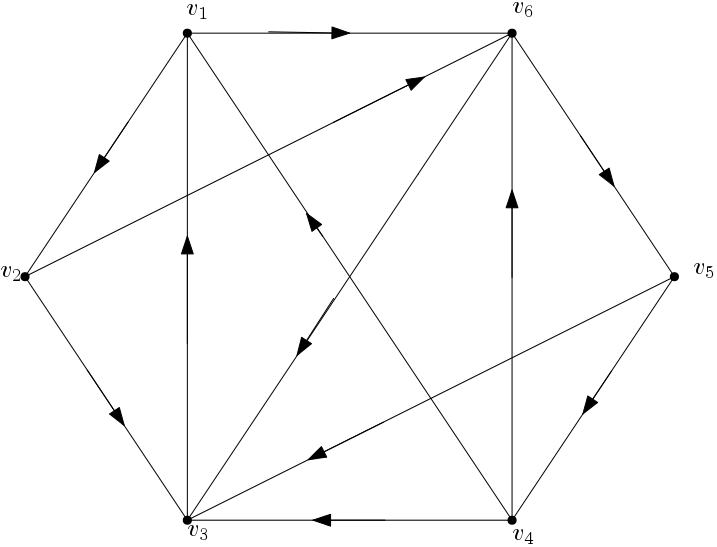
\includegraphics[width=0.4\textwidth]{2.6.png}\\
  \caption{}\label{fig:2.6}
\end{figure}
\textbf{解:}如果采用正向表的输入结构,则有\\
\begin{figure}[h]
  \centering
   \vspace{-10pt}
  % Requires \usepackage{graphicx}
  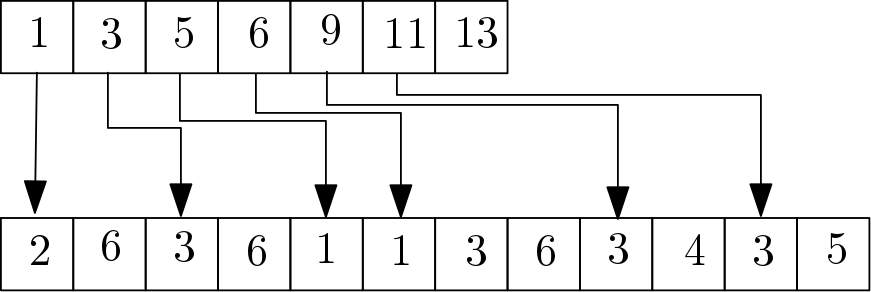
\includegraphics[width=0.4\textwidth]{2.6BFS.png}\\
  \caption*{}\label{} \vspace{-40pt}
\end{figure}
$\because \Gamma^{+}(v_1)={v_2,v_6},\therefore A_1={v_2,v_6}$。\\
$\because \Gamma^{+}(v_2)={v_3,v_6}$,\\
$\Gamma^{+}(v_6)={v_3,v_5},\therefore A_2={v_3,v_5}$。\\
$\because  \Gamma^{+}(v_3)={v_1},\Gamma^{+}(v_5)={v_3,v_4}$,\\
$\therefore A_3={v_4}$\\
\indent 从上例中可知,用BFS方法求两点间道路的计算复杂性是O(m)。
\end{sample}
\begin{figure}[h]
  \centering
  \vspace{-10pt}
  % Requires \usepackage{graphicx}
  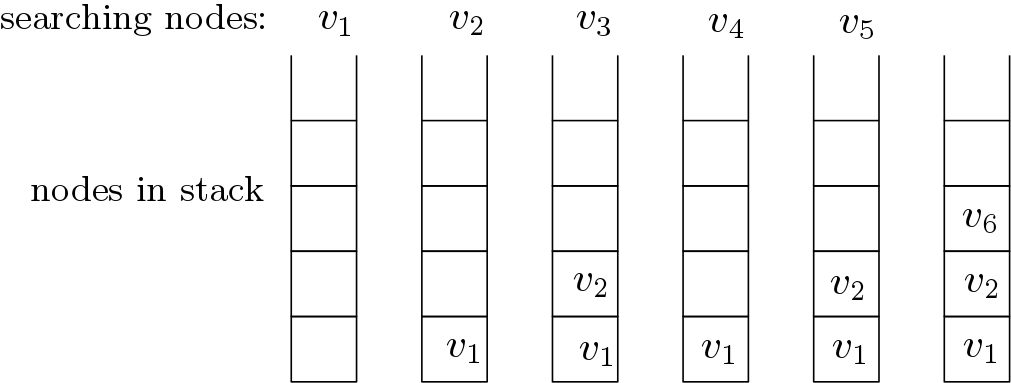
\includegraphics[width=0.5\textwidth]{2.6DFS.png}
  \caption{}\label{fig:2.7}\vspace{-25pt}
\end{figure}
\indent \textbf{深探法(DFS)}的特点与BFS截然不同。它从某一结点$v_0$开始,只查找$v_0$的某个直接后继$v_1$,记下$v_1$的父亲$v_0$,然后再找$v_1$的某个未搜索过的直接后继$v_2$。 依此类推。当从某个结点$v_j$无法再向下搜索时,退回到它的父亲$v_{j-1}$,然后再找$v_{j-1}$的另一个未查过的直接后继。形象地说,DFS的特点是尽量向下搜索,只有碰壁才回头。\\
\indent 采用栈结构以及前述的标记结点的方法可以完成DFS的搜索过程。\\
\begin{sample}
 用DFS方法找图2.6中$v_1$到$v_4$的一条道路。\\
 \textbf{解:}数据输入依然采用正向表。$v_1$的第一个直接后继是$v_2,v_1$进栈;$v_2$的第一个后继是 $v_3,v_2$进栈。$v_3$的后继是$v_1$,但已标记,故退栈。$v_2$的另一个后继是$v_6$,$v_2$进栈;$v_6$的第1个后继是已标记结点$v_3$,第2个后继是$v_5$,$v_6$进栈。$v_5$的后继是$v_4$。至此,已搜索到$v_1$到$v_4$的一条道路。整个搜索过程可用图2.7 形象地表示。其计算复杂性也是O(m)。
\end{sample}
\section{欧拉道路与回路}
\subsection{欧拉道路的引入}
\indent 1736年瑞士著名数学家欧拉(Leonhard Euler)发表了图论的第一篇论文“哥尼斯堡七桥问题”。这个问题是这样的:哥尼斯堡城被Pregel河分成了4部分,它们之间有7座桥。如图2.8 所示。当时人们提出了一个问题,能否从城市的某处出发,过每座桥一次且仅一次最后回到原处。欧拉的文章漂亮地解决了这个问题。他把4块陆地设想为4 个结点,分别用A、B、C、D 表示,而将桥画成相应的边,如图2.9。于是问题转化为在该图中是否存在经过每条边一次且仅一次的回路。欧拉的论文给出了解决这类问题的准则,并对七桥问题给出了否定的结论。\\
\begin{figure}[H]
  \centering
  % Requires \usepackage{graphicx}
  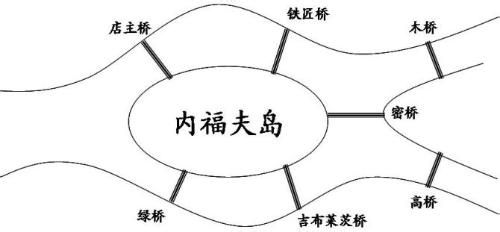
\includegraphics[width=0.5\textwidth]{2.3.1.jpg}
  \caption*{哥尼斯堡七桥}
\end{figure}
\begin{figure}[h]
  \centering
  \vspace{-10pt}
  \begin{minipage}[!ht]{.35\linewidth}
  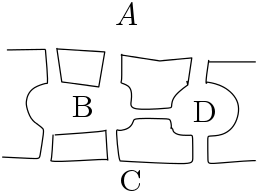
\includegraphics[width=1.0\linewidth]{2.8.png}
  \caption{}
  \end{minipage}
  \begin{minipage}[!ht]{.35\linewidth}
   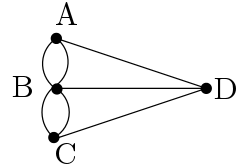
\includegraphics[width=1.0\linewidth]{2.9.png}
  \caption{}
  \end{minipage}
  \vspace{-25pt}
\end{figure}
\begin{defination}\K
给定无孤立结点的无向图G,经过图G每边一次且仅一次的迹称为\textbf{欧拉路}。无向连通图G=(V,E)中的一条经过所有边的简单回路(道路)称为G的\textbf{欧拉回路(道路)}。
\end{defination}
\begin{theorem}
无向连通图G存在欧拉回路的充要条件是G中各结点的度都是偶数。\\
\textbf{证明:}必要性。若G中有欧拉回路C,则C过每一条边一次且仅一次。对任一结点v来说,如果C经由$e_i$进入v,则一定通过另一条边$e_j$从v离开。因此结点v的度是偶数。\\
充分性。由于G是有穷图,因此可以断定,从G的任一结点$v_0$出发一定存在G的一条简单回路C。这是因为各结点的度都是偶数,所以这条简单道路不可能停留在$v_0$以外的某个结点,而不能再向前伸延以至构成回路C。
如果E(G)=C,则C就是欧拉回路,充分性得证。否则在G中删去C的各边,得到$G_1=G-C$。$G_1$可能是非连通图,但每个结点的度保持为偶数。这时,$G_1$中一定存在某个度非零的结点$v_i$,同时$v_i$也是C中的结点。否则C的结点与$G_1$的结点之间无边相连,与G是连通图矛盾。同样理由,从$v_i$出发,$G_1$中$v_i$所在的连通支内存在一条简单回路$C_1$。 显然$C\bigcup C_1$ 仍然是G的一条简单回路,但它包括的边数比C多。继续以上构造方法,最终有简单回路$C'=C\bigcup C_1\bigcup\cdots\bigcup C_k$,它包含了G的全部边,即C' 是G 的一条欧拉回路。\\
以上采用了构造性证明的方法,即证明过程本身就给出了问题求解的步骤。
\end{theorem}
\begin{sample}
试找出图2.10的一条欧拉回路。
\end{sample}
\begin{figure}[h]
  \centering
  % Requires \usepackage{graphicx}
  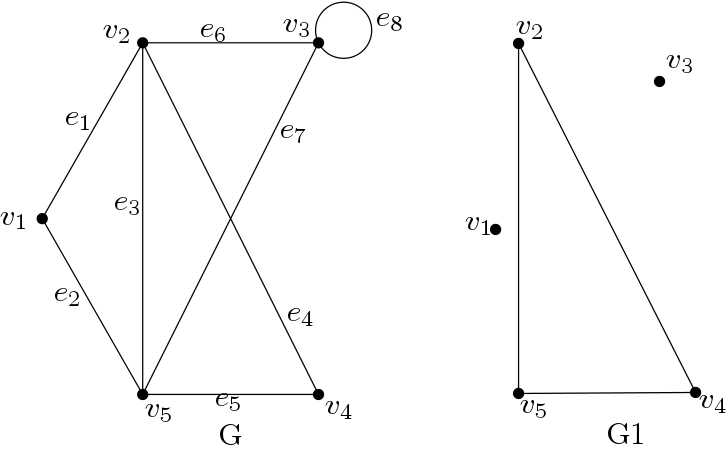
\includegraphics[width=0.5\textwidth]{2.10.png}\\
  \caption{}
\end{figure}
\indent 解:从任一点,比如$v_1$开始,可构造简单回路$C=(e_1,e_6,e_8,e_7,e_2)$。$G_1  =G-C$中的$v_2,v_5$度非零且是C中的结点,从$v_2$开始$G_1$中有简单回路$C1=(e_3,e_5,e_4)$。 因此 $C\bigcup C_1=(e_1,e_3,e_5,e_4,e_6,e_8,e_7,e_2)$包含了G的所有边,即是G的一条欧拉回路。
\begin{coro}
无向连通图G中只有2个度为奇的结点,则G存在欧拉道路。\\
\textbf{证明:}设$v_i$和$v_j$是两个度为奇数的结点。作$G'=G+(v_i,v_j)$,则G'中各点的度都是偶数。由定理2.3.1,G'有欧拉回路,它包含边$(v_i,v_j)$,删去该边,得到一条从$v_i$到$v_j$的简单道路,它恰好经过了G的所有边,亦即是一条欧拉道路。
\end{coro}
\begin{coro}
若有向连通图G中各结点的正、负度相等,则G存在有向欧拉回路。\\
其证明与定理2.3.1的证明相仿。
\end{coro}
\begin{sample}
七桥问题中既不存在欧拉回路也不存在欧拉道路。
\end{sample}
\begin{sample}
 设连通图G=(V,E)有k个度为奇数的结点,证明E(G)可以划分成k/2条简单道路。\\
 \textbf{证明:}由性质1.1.2,k是偶数。在这k个结点间增添k/2条边,使每个结点都与其中一条边关联,得到G',G'中各结点的度都为偶数。由定理2.3.1,G'中有欧拉回路C,这k/2条边都在C 上且不相邻接。删去这些边,得到k/2条简单道路,它们包含了G的所有边。亦即E(G)划分成了k/2条简单道路。
 \end{sample}
\begin{sample}
下图中,图G1是欧拉图;图G2不是欧拉图,但G2中存在欧拉路;图G3中即不存在欧拉回路,也不存在欧拉路。\\
\begin{figure}[h]
  \centering
  % Requires \usepackage{graphicx}
  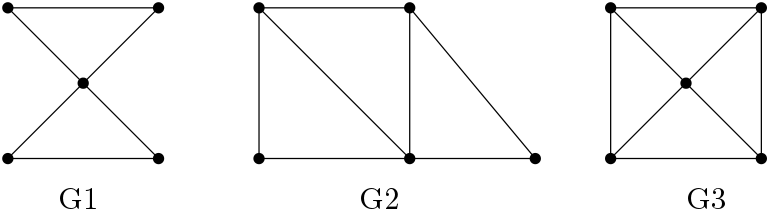
\includegraphics[width=0.6\textwidth]{2.f1.png}\\
  \caption*{}
\end{figure}
\end{sample}
\begin{sample}
下图中,图D1中既不存在有向欧拉回路,也不存在有向欧拉路;图D2是欧拉图;图D3不是欧拉图,但D3中存在有向欧拉路。
\begin{figure}[h]
  \centering
  % Requires \usepackage{graphicx}
  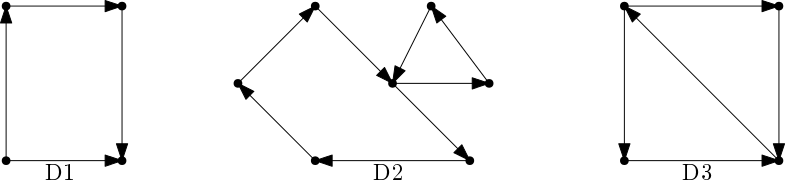
\includegraphics[width=0.6\textwidth]{2.f2.png}\\
  \caption*{}
\end{figure}
\end{sample}
\begin{sample}
蚂蚁比赛问题:甲,乙两只蚂蚁分别位于2.11图中的节点a,b处,并设图中的边长度是相等的。甲乙进行比赛:从它们所在的结点出发,走过图中的所有边,最后到达结点c处。如果它们的速度相同,问谁先到达目的地?\\
\begin{figure}[h]
  \centering
  \vspace{-20pt}
  % Requires \usepackage{graphicx}
  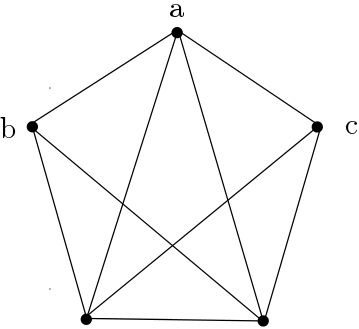
\includegraphics[width=0.3\textwidth]{mayi.png}
  \caption{}
\end{figure}
\textbf{解:}在图中仅有两个度数为奇数的结点b,c因而存在从b到c的欧拉通路,蚂蚁乙走到c只要一条欧拉通路,边数为9条。而蚂蚁甲要走完所有的边到达c,至少要先走一条边到达b,再走一条欧拉通路,因而它至少要走10条边才能到达c,所以乙必胜。
\end{sample}
\begin{sample}
一个编码盘分成16个相等的扇面,每个扇面分别由绝缘体和导体组成,可表示0和1两种状态,其中a,b,c,d四个位置的扇面组成一组二进制输出,如图2.12所示。试问这16个二进制数的序列应如何排列,才恰好能组成0000到1111的16组四位二进制输出,同时旋转一周后又返回到0000状态?\\
\begin{figure}[h]
  \centering
  \vspace{-10pt}
  \begin{minipage}[!ht]{.35\linewidth}
  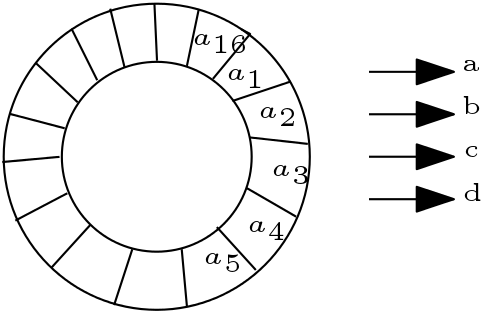
\includegraphics[width=1.0\linewidth]{2.11.png}
  \caption{}
  \end{minipage}
  \begin{minipage}[!ht]{.6\linewidth}
   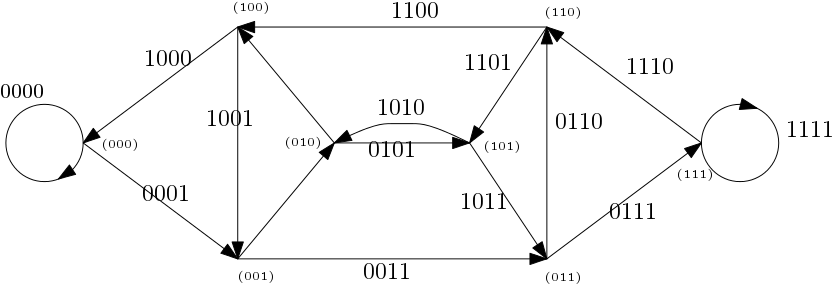
\includegraphics[width=1.0\linewidth]{2.12.png}
  \caption{}
  \end{minipage}
  \vspace{-20pt}
\end{figure}
\textbf{解:}我们发现如果从状态$a_1 a_2 a_3 a_4 (a_i=0或1)$逆时针方向旋转一个扇面,那么新的输出是$a_2 a_3 a_4 a_5$,其中有三位数字不变。因此可以用8个结点表示从000 到111 这8 个二进制数。这样从结点($a_{i-1} a_i a_{i+1}$)可以到达结点($a_i a_{i+1} 0$)或($a_i a_{i+1} 1$),其输出分别为($a_{i-1} a_i a_{i+1} 0$)和($a_{i-1} a_i a_{i+1} 1$),这样可以得到图2.13。它是有向连通图,共有16条边,且每结点的正、负度相等。由推论2.3.2,它存在有向欧拉回路。其中任一条都是原问题的解,比如(0000101001101111)就是一种方案。\\
\end{sample}
\subsection{科学家的故事-莱昂哈德$\centerdot$欧拉}
\begin{figure}[h]
  \centering
  % Requires \usepackage{graphicx}
  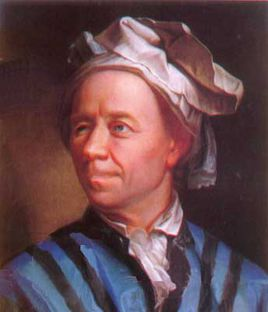
\includegraphics[width=0.3\textwidth]{oula.jpg}
  \caption*{莱昂哈德$\centerdot$欧拉}
\end{figure}
\indent 莱昂哈德$\centerdot$欧拉(Leonhard Euler ,1707 年4 月15 日~ 1783 年9 月18 日),瑞士数学家、自然科学家。1707 年4 月15 日出生于瑞士的巴塞尔,1783 年9 月18 日于俄国圣彼得堡去世。欧拉出生于牧师家庭,自幼受父亲的影响。13 岁时入读巴塞尔大学,15 岁大学毕业,16 岁获得硕士学位。\\
\indent 欧拉是18 世纪数学界最杰出的人物之一,他不但为数学界作出贡献,更把整个数学推至物理的领域。他是数学史上最多产的数学家,平均每年写出八百多页的论文,还写了大量的力学、分析学、几何学、变分法等的课本,《无穷小分析引论》、《微分学原理》、《积分学原理》等都成为数学界中的经典著作。在几何方面,欧拉解决了哥尼斯堡七桥问题,成为图论、拓扑学的滥觞。欧拉对数学的研究如此之广泛,因此在许多数学的分支中也可经常见到以他的名字命名的重要常数、公式和定理。\\
\indent 此外欧拉还涉及建筑学、弹道学、航海学等领域。\\
\begin{figure}[h]
  \centering
  % Requires \usepackage{graphicx}
  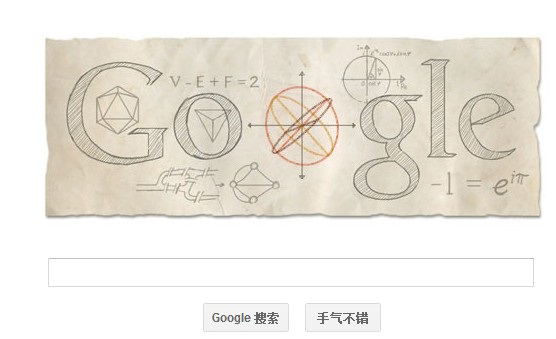
\includegraphics[width=0.6\textwidth]{oula1.png}
\end{figure}
\indent 2013 年4 月15 日是欧拉诞辰的306 周年,谷歌更换了首页涂鸦向这位数学天才致敬。在那天的谷歌涂鸦中,融入了许多欧拉的数学成就。

\section{哈密尔顿回路}
\subsection{哈密尔顿回路的引入} 一个包含一个无向图中所有的点的初级回路被称作\textbf{哈密尔顿回路}(Hamilton Cycle)。这源于1857年Sir William Hamilton发明的一种游戏——遍历一个正十二面体,不能经过一个点两次。一个含有哈密尔顿回路的图称作\textbf{哈密尔顿图}(Hamiltonian)。 事实上,在哈密尔顿之前,1759年,欧拉就已经研究了在一个国际象棋棋盘上骑士的遍历问题(Knight's Tour on a Chess Board)(图a给出了一个解)。如果我们对旅行商问题再加上一重限制,两个城市之间的旅行费用只有$1$ 和$\infty$ (也就是说不可能经过这条边),那么这个TSP问题就变成了这个图中所有的旅行费用为1 的边中是否存在一条哈密尔顿回路。然而,直到现在,即使这种TSP 问题的特殊情况仍然没有解决:没有有效算法构造图中的哈密尔顿回路,虽然是否真的有这样的算法也不知道。\\
\begin{figure}[H]
\centering
\subfigure[骑士遍历问题的一个解]{
\label{Fig.sub.h1}
\includegraphics[width=0.3\textwidth]{图0.png}}
\subfigure[正十二面体的一个哈密尔顿回路]{
\label{Fig.sub.h2}
\includegraphics[width=0.3\textwidth]{图1.png}}
\subfigure[赫歇尔图]{
\label{Fig.sub.h3}
\includegraphics[width=0.3\textwidth]{图2.png}}
\caption{正十二面体图(图b)是一个哈密尔顿图,而赫歇尔图(图c)则不是}
\label{Fig.lable}
\end{figure}
但是,边不交哈密尔顿回路问题现在我们已经可以很容易解决,这个问题在如下的例子中给出。\\
\begin{sample} {\K 约翰得到了n($\geq 2$)种宝石,他想把这n种宝石串成几条n-长的项链(每条项链中都含有每种宝石一颗),他希望自己串成的每条项链都本质不同,请问他最多能串出几条项链。两条项链\textbf{本质不同},当且仅当每种宝石相邻的宝石种类都不同。}\end{sample}
\textbf{解} 我们第一步估算上界:将n种宝石记作$v_0,v_1,v_2,\dots,v_{n-1}$, 作完全图$K_n$, 则此题转化为计算完全图$K_n$ 中边不交H回路计数问题;完全图中一共有$C_{n}^{2}=\frac{n(n-1)}{2}$条边,每条H回路长为n,所以至多存在$[\frac{C_n^2}{n}]=[\frac{n-1}{2}]$条边不交H回路。
\\第二步可以构造一个解。\\
$n=2k+1$时,如下图(Figure 2)将$v_1,v_2,\dots,v_{2k}$,排列在一个圆上,将$v_0$放在圆心。联结$(v_0,v_1,v_2,v_{2k},v_3,v_{2k-1},\dots,v_{k-1},v_{k+3},v_{k},v_{k+2},v_{k+1},v_0)$形成一条H回路;删除联结线,下面将$v_1,v_2,\dots,v_{2k}$命名为顺时针下一个点的名字,也即,将$v_{2k-1}$命名为$v_{2k}$,$v_{2k}$命名为$v_1$,$v_1$命名为$v_2$,$v_2$命名为$v_3$;重复执行联结操作,这样就得到k条边不交H回路。\\
$n=2k+2$时,$2\mid k$时,将$v_{2k+1}$插入$v_{\frac{k+2}{2}}$和$v_{\frac{3k+2}{2}}$的边中;$2 \nmid k$ 时,将$v_{2k+1}$ 插入$v_{\frac{k+3}{2}}$和$v_{\frac{3k+3}{2}}$的边中;依次就可以构造出k条边不交H回路。
综上,约翰可以串出$[\frac{n-1}{2}]$条本质不同的项链。
\begin{figure}[h]
 \centering
  % Requires \usepackage{graphicx}
  \includegraphics[width=0.5\textwidth]{图3.png}
  \caption{一种构造方案}\label{Fig.label}
\end{figure}

\begin{theorem} {\K $n\geq 2$的完全图$K_n$可以被分解成边不交哈密尔顿回路。}\end{theorem}
\begin{proof} 直接参照上例即可。 \end{proof}

\section{哈密尔顿回路的几个重要判定定理}
\begin{theorem} {\K 对于阶大于3的连通图G,能够满足$$\forall x, y \in G \wedge (x,y) \notin G \Rightarrow d(x)+d(y)\geq k$$
如果$k=n$那么G就是一个哈密尔顿图,而如果$k<n$那么G中就含有一条k-长路,以及一个长度至少为$\frac{k+2}{2}$ 的回路。}\end{theorem}
\begin{proof} 假设G不是哈密尔顿图,我们找到G中的最长道路P($=x_1x_2\dots x_l$)。由于P是最长道路,所以P是极长道路。考虑$$\Gamma(x_1)=\{x_j|(x_1, x_j) \in G\}, \Gamma^{+}(x_l)=\{x_{j+1}|(x_j, x_l) \in G\}.$$
我们可以断言这两个集合是不交的。否则就会产生回路,进而与G的连通性和非哈密尔顿图的性质违,这点留给读者自己证明。
那么由定理中的不等式,我们有$$k \leq d(x_1)+d(x_l)=\#\Gamma(x_1)+\#\Gamma^{+}(x_2)\leq l-1 \leq n-1.$$$\#S$ 表示集合S 的大小。
如果$k=n$,现在就已经产生了矛盾,G是一个哈密尔顿图。如果$k<n$,那么G中就存在一条长度为$l-1=k$的路。
如果再考虑$x_1$和$x_l$度的关系,不妨$d(x_l)>d(x_1)$,也即$d(x_l)\geq\frac{k}{2}$,我们就能够找到一个长度至少为$\frac{k+2}{2}$的回路了。\end{proof}

\begin{defination} \K 若$v_i$和$v_j$是简单图G的不相邻结点,且满足$d(v_i)+d(v_j)\geq k$,那么在G中增加边$(v_i, v_j)$,重复这个过程,直到不再有这样的结点对为止。最终得到的图称为G 的k-闭包,记作$C_k(G)$。\end{defination}

\begin{coro} \K 如果$\delta(G)\geq \frac{n}{2}$,那么图$G$是哈密尔顿图。\end{coro}

\begin{theorem} \K 图G是哈密尔顿图,当且仅当$C_n(G)$是;图G有哈密尔顿路,当且仅当$C_{n-1}(G)$有。\end{theorem}
\begin{proof} 这是\textbf{定理 0.2.1}的简单推论。\end{proof}

下面介绍一个中国数学家范更华给出的一个充分性判定条件。

\begin{theorem}[范更华]\K 对于一个2-连通图,如果对于任意一对距离为2的结点$x, y, d(x,y)=2$,都有$$max\{d(x),d(y)\}\geq \frac{n}{2},$$那么$G$是哈密尔顿图。\end{theorem}
\begin{proof}略\end{proof}

再介绍一个非常实用的平面图具有哈密尔顿圈的必要条件。(尽管我们还没有严谨地定义过平面图)
\begin{theorem}[Kozyrev and Grinberg] \K 如果一个平面图含有哈密尔顿圈$C$,用$f_k,g_k$表示$C$内部和外部的k 边形的数量,我们有$$\sum_{k\geq3}(k-2)(f_k-g_k)=0.$$\end{theorem}
这个定理可以很方便地证明一类平面图的非哈密尔顿性。

\begin{sample}[Grinberg图] Figure 3不含哈密尔顿回路。\end{sample}
\begin{proof} Figure 3中只有五边形、八边形和九边形。$$3(f_5-g_5)+6(f_8-g_8)+7(f_9-g_9)=0.$$所以,$$f_9\equiv g_9(mod 3)$$ 而$f_9+g_9=1$,所以不含哈密尔顿回路。\end{proof}
\begin{sample}[Grinberg图] Figure 3不含哈密尔顿回路。\end{sample}
\begin{figure}
  \centering
  \includegraphics[width=0.4\textwidth]{图4.png}
  \caption{Grinberg图}
\end{figure}
\begin{proof} Figure 3中只有五边形、八边形和九边形。$$3(f_5-g_5)+6(f_8-g_8)+7(f_9-g_9)=0.$$所以,$$f_9\equiv g_9(mod 3)$$ 而$f_9+g_9=1$,所以不含哈密尔顿回路。\end{proof}

\section{坚韧度与哈密尔顿性}
\begin{theorem} \K 如果图G=(V,E)是哈密尔顿图,那么$$\forall S \subset V \Rightarrow \sigma(G-S)\leq \#S,$$这里$\sigma(G-S)$表示$G-S$的分支数。\end{theorem}
\begin{proof} 找到哈密尔顿回路$C$,构造图$G'=(V',E')$,s.t.$$V'=V\cap C, E'= E.$$ 那么新图$G'$只包含这一个圈,如果去除掉$\#S$个点剩下就有最多$\#S$个分支,而原图的边更多一些,$$\sigma(G-S)\leq\sigma(G'-S)\leq\#S$$\end{proof}
这个定理很容易证明,然而由这个定理产生的对于哈密尔顿图充分条件的猜想,却很有意思。

\begin{defination}[Kozyrev and Grinberg] \K $t=min\frac{\#S}{\sigma(G-S)}$,则称G是t-\textbf{坚韧图}。\end{defination}

上面的定理表明:哈密尔顿图一定是1-\textbf{坚韧图}。
\\
\\
Chvatal认为图的坚韧性和哈密尔顿性应当存在双向的判定关系。提出了如下的猜想。
\begin{guess} \K 存在t满足任何t-坚韧图都是哈密尔顿图。\end{guess}
他给出了$\frac{3}{2}$-坚韧非哈密尔顿图。所以推测t应当等于2。因为这样的话就和Fleischner's theorem一致。

\begin{theorem}[Fleischner] \K 如果$G$是一个2-点连通图,那么$G^2$是哈密尔顿图。其中$G^2$ 中两点存在边当且仅当两点在$G$ 中距离小于等于2。\end{theorem}

之后,Thomassen发现了$t>\frac{3}{2}$的非哈密尔顿图,Enomoto等人发现了$(2-\epsilon)$-坚韧图对任意$\epsilon > 0$没有$2$- 因子。
\begin{defination} 一个$k$-因子是图的一个生成k-正则子图。\end{defination}

Enomoto的这个结论说明作为哈密尔顿图的判定依据的坚韧度至少为2。如果Chvatal的猜想成立,那么将证明两个开放了二十余年的猜想。
\begin{guess} \K 任意4-连通的点边对偶图是哈密尔顿图。\end{guess}
\begin{guess} \K 任意4-连通的不含$K_{1,3}$子图的图是哈密尔顿图。\end{guess}
近些年这两个猜想被证明是等价的。然而,人们却发现并不是每一个2-坚韧图都是哈密尔顿图。事实上,我们有如下的定理。

\begin{theorem}[D. Bauer et al] \K $\forall \epsilon > 0$,存在$(\frac{9}{4}-\epsilon)$- 坚韧的非哈密尔顿图。\end{theorem}

所以,关于作为哈密尔顿图的充分条件的坚韧度是否存在还是一个开放的问题。
\section{旅行商问题}
\subsection{旅行商问题}
\indent 上节讨论的哈密顿回路不涉及边的长度(权值)。但是在许多实际问题中,每条边都可以有自己的长度(权值)。如有若干个城市,任何城市之间的距离都是确定的,旅行商从某城市出发,必须经过每一个城市且只经过一次,最后回到出发城市。问如何事先确定好一条最短的路线,使其旅行的距离最短。这个问题便是著名的\textbf{旅行商问题(Traveling Salesman Problem)},又记作\textbf{TSP 问题}。在19 世纪,旅行商问题被数学形式化为给定一个正权完全图,求其总长最短的哈密顿回路。\\
\indent 即使是最朴素形式的旅行商问题也在很多领域有应用,如规划、物流、微电子元件的制造乃至DNA 序列上,在这些应用中,城市的概念被替换为顾客、销售点、DNA 片段等,距离的概念被替换为旅行时间、代价或者DNA 片段之间的相似性。\\
\indent 但是容易知道,n 个节点的完全图存在1/2 (n-1)! 个不同的H 回路。如果使用穷举搜索法对TSP问题进行求解,即使使用每秒能进行十亿亿次浮点数运算的“神威·太湖之光”超级计算机,对于30 个点的情况也需要$1.4\times10^4$个世纪。事实上在20 世纪70 年代旅行商问题就已被证明是NP-complete问题。\\
\indent 在1948 年美国兰德(Rand)公司向推动旅行商问题解决者颁发奖励后,旅行商问题成为近代组合优化领域的一个著名问题。而在当时兰德公司的三位专家通过手工和计算机相结合的办法,创造了周游49 个城市的纪录。\\
\indent 目前对于旅行商问题的求解方法主要分为两类:精确算法与近似算法。\\
\indent 其中精确算法主要包括穷举法(复杂度为O(n!)),和动态规划法(复杂度为O($n^2 2^n$))等。通过对于穷举法加入剪枝技巧我们还可以得到分支与界法(branch-and-bound method,又称作分支限界法)。在上个世纪60 年代,理查德$\cdot$卡普(Richard Manning Karp)通过分支与界法把旅行商问题的纪录提高到了65 个城市。而目前确定性算法的最高记录是2006 年的85900 个城市,其使用的方法是branch-and-bound 和branch-and-cut 算法。\\
\indent 在本节中我们将介绍一个确定性算法\textbf{分支与界法}和一个近似算法\textbf{便宜算法(又称最近邻算法)}。
\subsection{分支与界法}
\indent \textbf{分支与界法(branch-and-bound method,又称作分支限界法)}是解决旅行商问题的一个确定性算法。算法基本思想是对边按权值排序后,按顺序搜索所有可能成为解的H 回路,并通过已有解的上界对搜索树进行剪枝。其算法伪代码如下:\\
\begin{algorithm}
\renewcommand{\algorithmicrequire}{\textbf{Input:}}
\renewcommand\algorithmicensure {\textbf{Output:} }
    \caption{Huffman算法}
    \label{alg:6}%这个是编号
    \begin{algorithmic}[1]
      \label{alg:babm}  %state命令是开始算法,这是会有默认的编号产生
      \STATE 对t$(t \ge 2)$个权值进行排序,使得
      \begin{displaymath}
      \qquad
        w_{i1} \leqslant w_{i2} \leqslant ... \leqslant w_{it}
      \end{displaymath}
      \STATE 计算$w_i=w_{i1}+w_{i2}$作为中间结点$v_i$的权,$v_i$的左儿子是$v_{i1}$,右儿子是$v_{i2}$。在权序列中删去$w_{i1},w_{i2}$,加入$w_i$,$t\gets t-1$。若t=1,结束。否则转(1)。
        % \FOR {...用公式或者文字描写for语句}
        %    \STATE  %for里边的具体内容
        % \ENDFOR   %用endfor来结束for语句
    \end{algorithmic}
\end{algorithm}



































\end{document}
